\documentclass[cn,fancy,blue,11pt]{elegantbook}


\title{几何的公理化方法}
\subtitle{几何三部曲·第一卷}

\author{F.~Borceux}
\translator{宋宁}
\institute{山东理工大学}
\date{\today}


\equote{我们必须知道,我们必将知道 ------ 大卫·希尔伯特}

\logo{timg.jpg}
\cover{cover.jpg}

\usepackage[authoryear]{gbt7714}
\usepackage{framed} 

\begin{document}

%\newtheorem{problem}{问题}[section]

\maketitle

\tableofcontents

\mainmatter
\hypersetup{pageanchor=true}

\chapter{前希腊时代的几何}

在受到古希腊几何的系统性工作影响之前,
各个古代文明相继产生了早期的几何思想.
这个非常简短的一章将概括地介绍这些早期的几何思想.
所以,``前希腊''这个词应该理解为``在受到希腊影响之前''.

在``前希腊时代的几何''这一章里,
我们所见识到的几何工作来自古埃及和古巴比伦.
这是因为在前希腊时代,
只有这两个古文明的手写几何资料被保留到了当代
(译者注:虽然同时期古中国和古印度的几何也应该产生了很高的成就,
但是确实没有足够的出土文物的支撑,
比如,我们一般认为的我国最早的数学专著《周髀算经》,
我们甚至无法确定其成书年代,所以作者的解释也是合理的).

\section{史前时代}

在史前时代,人类还没有发明文字.
所以,知识只能依靠口头传播.
而今我们已经无法听到那些声音了.
因此史前时代的几何正如史前时代人类生活的其他方面一样,
我们对其知之甚少.
我们所能做的只是依赖考古发现,
去尝试解读各种洞穴壁画和其他出土文物.

最早的几何图画可以追述到公元前25000年.
它们暗示着当时的人类已经理解了图形对称和全等的概念.
同时代其他一些出土文物则展示出早期算术(比如计数)发展的迹象.

特别有趣的是图\ref{fig:1-1}中这幅图画.
它似乎表明史前艺术家并不只关注于绘画是否漂亮,
其实作者更想强调这是他/她的一个数学发现.
事实上,从图画中,我们立即可以发现:
\begin{itemize}
	\item 如果将三角形的边长变为原来的2倍,会导致其面积变为原来的4倍;如果将边长变为原来的3倍,会导致面积变为原来的9倍;
	\item 数一下每行上的小三角形个数,我们会发现:\[1=1,~~~~1+3=4,~~~~1+3+5=9.\]
\end{itemize}

\begin{figure}[htbp]
	\centering
	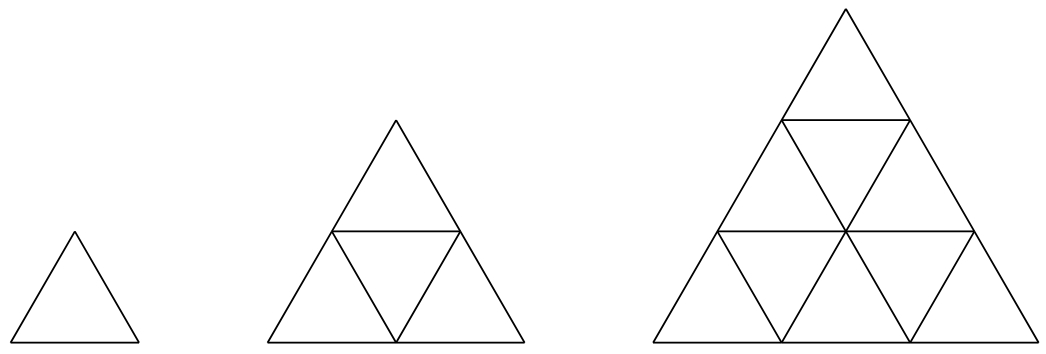
\includegraphics[width=0.6\textwidth]{fig-1-1.jpg}
	\caption{\label{fig:1-1}}
\end{figure}

这个目前已知最古老的几何手稿涉及到两个一般结果:
\begin{itemize}
	\item 边长乘以$n$会导致面积乘以$n^2$;
	\item 前$n$个奇数之和是$n^2$.
\end{itemize}
那么这位史前艺术家在多大程度上能意识到这些``定理''呢?我们不得而知.

一种传统观点认为,算术和几何源自于我们祖先的某些宗教仪式.
他们对一些能提高他们法力的图形和数字非常痴迷.
通过将这些有神力的图形和数字引入他们的宗教仪式,
他们或许就能获得神灵的保佑.

希罗多德(约公元前484年-约公元前425年)则提出了另一个传统观点.
他认为几何学的产生是因为反复无常的尼罗河.
希罗多德记载,
传奇法老辛努塞尔特(公元前1300年前后)
曾经在贵族之间分配土地.
尼罗河河谷一年一度的洪水,
虽然带来肥沃的土壤,
但也引发了许多戏剧性事件,
这就要求必须设计出切实可行的办法,
在每次洪水过后,能追溯每块田产的界限.
这些方法主要是基于三角剖分,
还要借助勾股定理的某些特例来构造直角三角形.
例如,三边长度分别为3,4,5的三角形为直角三角形,
这似乎至少在公元前2000年就已经知道了.

但是从数学早期发展来看,
尼罗河河谷并不占据的绝对优势,
即使在非洲,它也并不突出.
1950年,在刚果发现的伊尚戈骨骼化石,
可以追溯到公元前22000年前后,
是某种数学活动的最古老证据之一.
类似考古发现广泛地出现在欧洲、印度、中国、美索不达米亚等地.
这表明在这一时期不同发展层次的数学思想在世界各地广泛地出现了.

然而,到目前为止,羞怯的史前时代几何仍然很少在世人面前揭开她神秘的面纱.

\section{埃及}

我们已知最古老的数学纸草书是所谓的``莫斯科纸草书'',
它很可能写于公元前1850年.
但是我们对于远古埃及数学的了解却主要来自于公元前1650年前后的一位抄写员阿美斯,
他抄写了一个更大的纸草书.
该纸草书记录了许多算术和几何问题及其解答,
而根据阿美斯本人的记载,这些问题的设计可以追溯到公元前2000年前后.

莫斯科纸草书也称为戈列尼雪夫数学纸草书.
它是俄罗斯埃及学家戈列尼雪夫于1893年在底比斯收购的.
这个纸草书后来收藏在莫斯科普希金国家艺术博物馆,直到现在.
阿美斯纸草书也称莱茵德纸草书,
它是苏格兰文物收藏家莱茵德于1858年在卢克索收购的.
这片纸草书在盗掘法老拉美西斯二世陵墓时被发现,
现存于伦敦大英博物馆.

举例来说,阿美斯纸草书的问题51求证:
\begin{framed}
	等腰三角形的面积等于高乘以底的一半.
\end{framed}
而解决方法是如图\ref{fig:1-2}所示的``割补法''.
也就是沿着该三角形的高将三角形剪开,
然后将其中一片上下颠倒再粘回去,这样就得到了右边的矩形.
\begin{figure}[htbp]
	\centering
	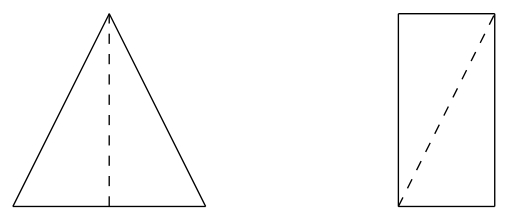
\includegraphics[width=0.6\textwidth]{fig-1-2.jpg}
	\caption{\label{fig:1-2}}
\end{figure}
类似的论证方法也出现在问题52中,这个问题求证:
\begin{framed}
	等腰梯形的面积等于高乘以两底和的一半.
\end{framed}
证明如图\ref{fig:1-3}所示,
至少在那个时代,这确实是一个证明,
而且是一个基于图形全等的证明.
\begin{figure}[htbp]
	\centering
	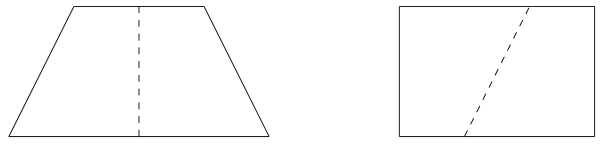
\includegraphics[width=0.6\textwidth]{fig-1-3.jpg}
	\caption{\label{fig:1-3}}
\end{figure}

然而,严格地从数学术语来讲,埃及人并没有``定理''或``形式证明''是什么的概念.
尤其是,他们并不能区分什么是精确解和近似解.
例如,埃及文献中会使用下列奇怪的方法计算四边形的面积:
\begin{framed}
	任意四边形的面积等于对边和的一半的乘积.
\end{framed}
这显然与阿美斯纸草书的问题52矛盾.
但这似乎没让谁觉得不对.
而且更令人吃惊的是由这个法则得到的推论:
\begin{framed}
	三角形的面积等于一边的一半乘以另外两边和的一半
\end{framed}
这与阿美斯纸草书的问题51又矛盾了一把.
但是这里却有一个最牛逼的惊喜:埃及人会把三角形看成一种特殊的四边形,其一边长度为零.
当时的人们已经可以这样抽象地思考问题,这是我们所难以想象的.

纸草书上也会考虑圆的面积的问题.
阿美斯纸草书的问题50就断言:
\begin{framed}
	直径为9的圆与边长为8的正方形面积相等.
\end{framed}
从圆的面积公式来看,这一断言相当于认为
\[\pi=\frac{256}{81}\approx3.16\]
这相当牛逼!
对比来看,
《圣经》中记载直径为10的圆的周长为30,
这相当于认为$\pi=3$.
但是,埃及人似乎并没有意识到$\pi$是所有的圆所共有的一个常数,不论这个圆多大.
稍后我们再来聊聊这样一个常数$\pi$在古人看来是个神马东东(见2.6节).

另一方面,古埃及人发现了圆的面积与周长的关系.
\begin{framed}
	圆的面积与周长之比等于一个正方形的面积与周长之比,这个正方形的边长为圆的直径.
\end{framed}
如果设该圆的半径为$R$,那么这个论断用现代代数符号来表达那就是:
\[\frac{\pi R^2}{2\pi R}=\frac{(2R)^2}{4(2R)}.\]

埃及人还知道如何计算金字塔的体积:
\[\frac{1}{3}\times\textrm{底}\times\textrm{高}.\]
我们并不知道他们是怎么发现这个公式的,
尽管我们能想象他们会怎么用这个公式.

阿美斯纸草书的问题56还探讨了三角形的相似性:
\begin{framed}
	对应边成比例的直角三角形的对应角相等.
\end{framed}
\begin{figure}[htbp]
	\centering
	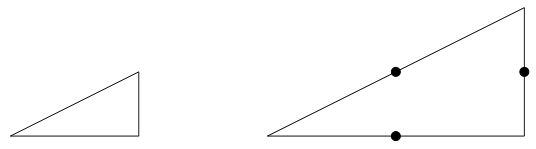
\includegraphics[width=0.6\textwidth]{fig-1-4.jpg}
	\caption{\label{fig:1-4}}
\end{figure}
在这问题(如图\ref{fig:1-4}所示)中,
两个三角形的内角使用余切进行了测量.
这种结果在建造金字塔时非常有用,
它可以用来保持斜面的倾斜程度.

\section{美索不达米亚}

咱们现在离开尼罗河谷地,去美索不达米亚的幼发拉底河和底格里斯河谷地瞧瞧.
把象形文字抛在脑后,瞅瞅楔形文字(公元前3000年).
它们通常刻在泥板上,而不是纸草上.
这就保证了有大量文献能完好地保存几个世纪.

这些巴比伦人相当擅长代数和天文学.
他们能解决一次、二次甚至某些更高次的代数方程.
我们在时间和角度上所用的六十进制就是从他们那里继承的.
一些泥板上还记录了三角学,给出角的正割值.

但是,和埃及人一样,美索不达米亚人不能区分精确解和近似解.
有块泥板给出了前七个正多边形的近似面积.
而对于圆而言,
它声称:圆内接六边形的周长为这个圆的周长的$\frac{24}{25}$.
用现代符号来说,就是
\[6R=\frac{24}{25}2\pi R\]
由此可得
\[\pi=\frac{25}{8}=3.125.\]

另一个泥板声称棱锥的体积等于一半的底面面积乘以高!
但埃及人已经得到了正确的公式(三分之一而不是二分之一).
可见,从几何学的发展来看,两个文明的交流很有限.

事实上,巴比伦人在毕达哥拉斯出生以前一千年就已经广泛地使用了勾股定理
(译者注:西方人习惯称勾股定理为毕达哥拉斯定理).
一块泥板上有这样一个题目:
\begin{framed}
	一个梯子斜靠在墙上.梯子顶端沿着墙滑动了$3$个单位,梯子底端就会沿着地面滑动$9$个单位.那么梯子有多长?
\end{framed}
另一个泥板则解释了如何使用勾股定理求圆内接弦的弦心距.

与我们长期以来的想象相反,在整个古代,
美索不达米亚的几何发展与埃及相比有过之而无不及.
尤其是,勾股定理的系统性使用,
与埃及纸草书在这方面的明显欠缺形成了鲜明的对比.

巴比伦人也已经知道了如下定理.
\begin{theorem*}{}{}
	半圆的所对的圆周角是直角.
\end{theorem*}

这个定理习惯上归功于一千年以后的希腊数学家泰勒斯,
而埃及人则根本不知道这个事实.
那么巴比伦人是如何知道并证实这个结果的?我们不得而知.
他们很可能是通过实验观察到了如下结论(如图所示):
\begin{itemize}
	\item 设$\angle ABC$是半圆所对一个圆周角角.
	\item 设$B'$是$B$关于$O$的对称点.
	\item 这样就形成了四个等腰三角形,其中有两对全等.
	\item 所以$\angle ABC=\angle BCB'=\angle CB'A=\angle B'AB$.
	\item 由对称性可知,四边形$ABCB'$的对边等长.
	\item 四边形$ABCB'$的对角线相等.
\end{itemize}
这些理由足以说服巴比伦人相信这个四边形是矩形
(译者注:巴比伦人和埃及人都没有``证明''的概念,所以只能通过经验说服他们相信某个事实).

\section{问题}

\begin{problem}
	求证一个立方体是三个等体积棱锥的并,从而立即得到棱锥的体积公式.
\end{problem}

\begin{problem}
	考虑一个棱锥,其底面是一个正方形,其锥顶的正交射影恰好是底面的中心.
	通过割补法推导这个棱锥的体积公式.
\end{problem}

\begin{problem}
	证明巴比伦人的梯子问题有无数个解.
\end{problem}

\section{练习}

\begin{exercise}
	使用割补法推导平行四边形的面积公式.
\end{exercise}

\begin{exercise}
	使用割补法推导任意三角形的面积公式.
\end{exercise}

\begin{exercise}
	使用割补法推导任意梯形的面积公式.
\end{exercise}

\chapter{希腊几何的先驱}

本章开始了数学史上黄金篇章的探讨.
这一时代是数学真正的开端,
不仅是因为这一时期涌现出的数学成果,
更重要的是这些成果告诉我们,
数学的演绎推理诞生了.

欧几里得的著作《原本》(大约公元前300年)被看作学习希腊几何的经典教材.
这部著作是一项伟大的成就,
我们将把下一章完全贡献给它.
可是那些被欧几里得系统化组织和继承起来的成果最初源于何处,
我们却知之甚少,甚至无从知晓.

而在本章,我们将关注于比欧几里得更早的希腊几何学家.
在他们的时代,几何学的基础正在被建立起来,
他们因而也遇到了各种极富挑战的问题.
在解决这些问题的过程中,
他们慢慢收集着各种必需的资料,
最终由欧几里得总结而集其大成,
并进一步由阿基米德、阿波罗尼乌斯、帕普斯和其他人将之发扬光大.
那些欧几里得之前的先驱们从他们的前辈那里学到了关于三角形和圆的基础知识.
他们究竟确切地知道些什么?
谁最早从这些经验知识中写出了第一个形式化的证明?
哪些论证方法和论据被用来支撑这个证明?
这些我们都不得而知.
尽管如此,必要时为了避免重复,
我们将在本章自由地使用这些结果;
如果你希望看到这些结论的系统化论述,
我们将在下一章呈现.

在希腊数学的最伟大的几何难题中,
每个人都听说过圆化方问题,
可能也听说过倍立方问题和三等分角问题.
对这些问题的最终(否定)回答直到两千年以后才出现!
但是,为了尝试解决这些问题,
几何学家做出了许多不成功的努力.
正是这些努力导致人们发现了很多技巧和结果,比如圆锥曲线的相关结论,
这远比那些问题重要得多.

希腊几何还有一个成就,虽然这个成就很少有人关注,
但是对几何学甚至数学日后的发展具有极其重要的基础作用.
这就是不可公度量和穷竭法.
用现代的数学术语来说,前者相当于从几何的视角发现了无理数和实数,
后者则是对曲线的极限进行研究的方法.
它们与戴德金分割的思想相差甚微,
简单地说,差别在于:希腊几何学家只是不称它们是数而已.
可以说,在戴德金出生的23个世纪之前,
戴德金分割的方法就已经被希腊人思考和使用了,
这是最引人瞩目的.

\section{米利都的泰勒斯}

米利都的泰勒斯(约公元前620年-约公元前546年)是我们目前所能接触到的文献中明确提到的第一位希腊几何学家.
然而这些文献仅仅依赖传说,因为它们都是泰勒斯死后几百年才写下的.
因而,关于泰勒斯和他的成就一直存在着争议.

在游历埃及和美索不达米亚时,泰勒斯接触到了大量重要的科学知识.
当这些知识与泰勒斯卓越的头脑相遇时,
就仿佛种子播种到了肥沃的土壤一样,结出了累累硕果.
正如泰勒斯被后人誉为已知的第一个希腊几何学家一样,
在他游历期间细心收集起来的很多结果也被人们认为是他的创造,例如
\begin{itemize}
	\item 半圆所对的圆周角是直角.
	\item 等腰三角形的底角相等.
	\item 两直线相交对顶角相等.
\end{itemize}
当然,这些结果在泰勒斯之前很早就被发现了,
但是泰勒斯仍然是对它们进行形式化证明的第一人.

确实,传说将一个重要功绩归功于泰勒斯,
那就是:他是第一个用逻辑和推理证明他的定理的人.
一些非常基础的结果归功于他,例如
\begin{itemize}
	\item 直径将圆分割了全等的两半.
	\item 如果一个三角形的两条边与另一个三角形的两条边相等并且这两边夹角也相等,那么这两个三角形全等.
\end{itemize}
他有可能尝试从这些基本结论出发论证更复杂的结果.
然而不幸的是,没有现存与泰勒斯的工作相关的资料能证明这一点.
因此,我们必须小心翼翼地从各种传说故事中分辨出真相,
这些传说将泰勒斯描述成数学家、商人、政治家、天文学家...以及独身主义者.

亚里士多德(公元前384年-公元前322年)曾写道:
\begin{framed}
	对于泰勒斯,最基本的问题不是``我们知道什么?''而是``我们怎么知道的?''
\end{framed}
这种对于完美的追求导致希腊几何学家创造出两千年都难以磨灭的工作,
被认为是数学思想的最高成就.

然而在今天,泰勒斯的名字首先是与下面这个结果联系在一起:

\begin{theorem*}{泰勒斯截线定理}{}
	对任意两条直线$d$和$d'$以及四条与$d,d'$相交的平行线$d_1,d_2,d_3,d_4$(如图\ref{fig:2-1}所示),
	如下比例式成立:
	\[\frac{AB}{A'B'}=\frac{CD}{C'D'}.\]
\end{theorem*}

\begin{figure}[htbp]
	\centering
	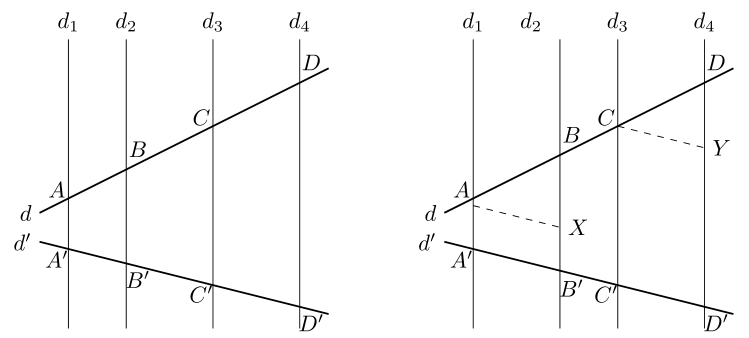
\includegraphics[width=0.6\textwidth]{fig-2-1.jpg}
	\caption{\label{fig:2-1}}
\end{figure}

(译者注:对$d$和$d'$,所有平行于同一直线的平行线会给出$d$到$d'$的一个一一对应,
这个一一对应叫做$d$到$d'$的一个\textbf{仿射对应},仿射对应下的像称为\textbf{仿射投影},
比如上图中$A'$是$A$的仿射投影,线段$A'B'$是$AB$的仿射投影.
泰勒斯定理实际上说明,三点单比是仿射对应下的不变量,这是仿射几何学的基础之一.)
\vskip 10pt

那么泰勒斯是否证明了这个定理?如果是,那他是怎么证明的?我们仍然不得而知.
传说声称泰勒斯使用了这个结果测量了胡夫金字塔.
对于这个定理,我们已知最古老的证明有时被称为``石器时代的证明'',
因为它是受到了大约公元前2500年的一幅新石器时代的石刻画的启发而做成的,
但是它仍然出现在19世纪的一些教材中.

\begin{itemize}
	\item 首先考虑图\ref{fig:2-1}右侧的特殊情况,即$AB=CD$的情况.
	\item 作$AX,CY$平行于$d'$.
	\item 三角形$AXB$与三角形$CYD$全等,因为$AB=CD$以及平行关系.
	\item 因此$AX=CY$;由于$AXB'A'$和$CYD'C'$是平行四边形,所以$AX=A'B',~CY=C'D'$,因此$A'B'=C'D'$.
\end{itemize}
这就证明了\[AB=CD~~~\Longrightarrow~~~A'B'=C'D'.\]

现在我们回到一般情况.
在直线$d$上选择一个单位长度$\epsilon$,
要求它足够小以至于可以同时测量$AB$和$CD$.
我们设$AB$的长度为$n\epsilon$,
$CD$的长度为$m\epsilon$.
由前面的特殊情况可知,
$d$上所有长为$\epsilon$的线段在$d'$上的仿射投影等长,记这个长度为$\epsilon'$.
于是$A'B'$和$C'D'$的长度分别为$n\epsilon'$和$m\epsilon'$.
由此可知:
\[\frac{AB}{A'B'}=\frac{n\epsilon}{n\epsilon'}=\frac{\epsilon}{\epsilon'}
=\frac{m\epsilon}{m\epsilon'}=\frac{CD}{C'D'}.\]
这样我们就完成了``证明''.

\vskip 10pt
(译者注:
\begin{itemize}
	\item 本书不使用$\triangle ABC$表示三角形$ABC$,因为这个符号容易和本书后面的一个符号相混淆.
	\item 泰勒斯截线定理,在我国中学教学中也称为``平行线分线段成比例定理''.
	\item 注意作者的最后一句话``这样我们就完成了`证明''',作者在``证明''二字上加了引号其实颇有深意.
	\item 因为这个证明隐藏着一个巨大的漏洞,那么就是$\epsilon$很可能并不存在.
	\item 比如说如果$AB=1$且$CD=\sqrt{2}$,换句话说这里的$\epsilon$可能是不可公度量.
	\item 真正严格的证明,应该按$AB$与$BC$的比例为有理数和无理数分为两种情况,先证有理数情况,再用有理数情况逼近无理数,可以用反证法表述.
	\item 所以说,不可公度量在数学史上出现也许并不是某个学生的灵光一现,而是证明比例问题时的一种必然.
	\item 另外,原著在此处有一个笔误,翻译时已经更改.
\end{itemize}
)

\begin{figure}[htbp]
	\centering
	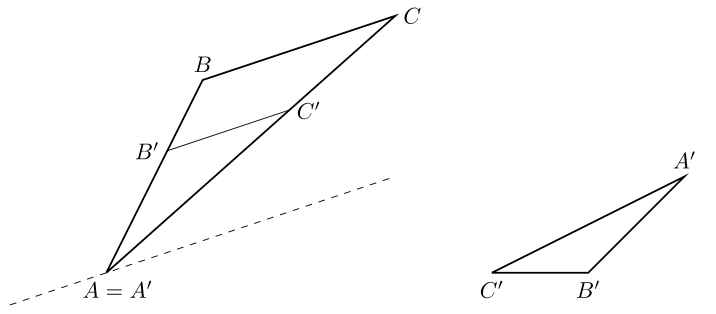
\includegraphics[width=0.6\textwidth]{fig-2-2.jpg}
	\caption{\label{fig:2-2}}
\end{figure}

当然,我们今天已经知道,这个证明中有一个巨大的瑕疵:用来同时测量$AB$和$CD$的单位长度$\epsilon$.
要想让$\epsilon$成为$AB$和$CD$之比,我们会遇到如图2.16所示的困境.

泰勒斯定理的主要应用在于相似三角形理论(见图\ref{fig:2-2}):

\begin{corollary*}{}{}
	如果两个三角形三组对应角分别相等,那么它们的对应边比例相等.
\end{corollary*}

确实,如果两个三角形$ABC$和$A'B'C'$有相等的角,
分别是$\angle A$和$\angle A'$、
$\angle B$和$\angle B'$、$\angle C$和$\angle C'$,
将三角形$B'A'C'$移动到三角形$BAC$的位置,并使$\angle A$和$\angle A'$重合,
因为$\angle B$和$\angle B'$相等,$\angle C$和$\angle C'$相等,
所以$BC$和$B'C'$平行,
因此,由泰勒斯定理可知:
\[\frac{AB}{A'B'}=\frac{AC}{A'C'}.\]
类似地,将$\angle B$与$\angle B'$重合,会得到:
\[\frac{BA}{B'A'}=\frac{BC}{B'C'}\]
因而
\[\frac{AB}{A'B'}=\frac{AC}{A'C'}=\frac{BC}{B'C'}.\]

这个关于相似三角形的结果在希腊几何发展中扮演了一个至关重要的角色.

\section{毕达哥拉斯和黄金比}

毕达哥拉斯(约公元前580年-约公元前500年),
与泰勒斯一样,在游历埃及和美索不达米亚时学习了几何学.
尤其是,他学到了在他出生前一千年就已经在埃及广为人知的毕达哥拉斯定理(勾股定理).

\begin{theorem*}{毕达哥拉斯定理(勾股定理)}{}
	给定一个直角三角形,以两直角边为边的正方形的面积之和等于以斜边为边的正方形的面积
	(如图所示\ref{fig:2-3}).
\end{theorem*}

\begin{figure}[htbp]
	\centering
	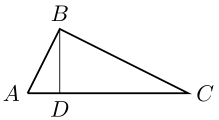
\includegraphics[width=0.2\textwidth]{fig-2-3.jpg}
	\caption{\label{fig:2-3}}
\end{figure}

非常确定的是,毕达哥拉斯知道或者可能自己给出了这个定理的一个形式化的证明.
如下证明基于泰勒斯定理关于相似三角形的推论,这个证明如今广为人知,也很可能为毕达哥拉斯所知.

直角三角形$ABC$和直角三角形$ADB$有一个公共角$\angle A$,
因此它们相似,由此可知,
\[\frac{AB}{AD}=\frac{AC}{AB},~~~\frac{BC}{AC}=\frac{DC}{BC}.\]
因此\[AB^2+BC^2=AD\cdot AC+DC\cdot AC=(AD+DC)\cdot AC=AC\cdot AC=AC^2.\]
(译者注:此处原作者有一个小小的笔误)

我们还是回到古希腊.
毕达哥拉斯建立了一个包含哲学和数学问题的宗教世界.
当时有这样一个潜规则(现在有时候还这样吗?):
追随者发现的结果要归于领导者名下,哪怕他已经死了!
所以当我们提到毕达哥拉斯的成果的时候,
更合理的说法是他的学派的成果.

毕达哥拉斯学派认为某些数和某些几何图形,尤其是正则图形,具有神奇的美德.
一些历史学家认为他们已经知道了五种正多面体:
正四面体、正六面体、正八面体、正十二面体和正二十面体.
但是没有证据能证明此事.

另一方面,毕达哥拉斯学派的标志是已经被巴比伦人知晓的正五角星(如图\ref{fig:2-4}所示),这是可以确定的.
希腊几何学家很可能通过仔细观察这个几何图形发现了所谓\textbf{黄金比}.
确切地说,这需要灵活使用圆周角的性质,这些性质将在下一章讨论.
至于毕达哥拉斯是否知道这些结果,或者他是否使用了其他证明方法,我们不得而知.

\begin{figure}[htbp]
	\centering
	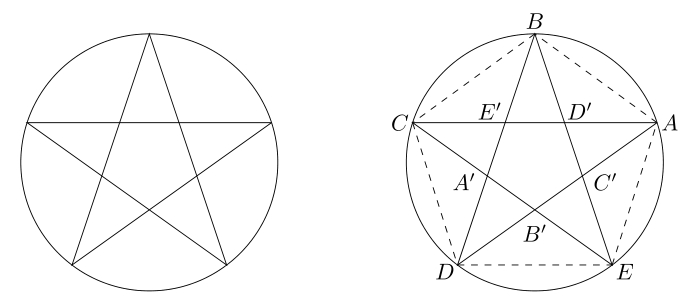
\includegraphics[width=0.6\textwidth]{fig-2-4.jpg}
	\caption{\label{fig:2-4}}
\end{figure}

圆上同一个弦所对的圆周角相等.
因此$\angle BCA=\angle BDA$.
再结合正五角星的对称性可得,
\[\angle BCD'=\angle BCA=\angle BDA=\angle CEB.\]
再加上公共角$\angle CBD'=\angle CBE$,
所以,三角形$BCD'$与$CEB$相似.
又因为$CEB$是等腰三角形,
所以$BCD'$也是等腰三角形.
由相似三角形的边成比例可知:
\[\frac{BE}{CD'}=\frac{BC}{BD'},\]
再次借助正五角星的对称性并考虑到三角形是等腰的,有
\[\frac{AC}{CD'}=\frac{AC}{BC}=\frac{AC}{CD'}=\frac{BE}{CD'}\frac{CD'}{AD'}.\]
这个等式可以概括为
\begin{framed}
	点$D'$将线段$AC$分割为两部分,使得整个线段与较长部分之比等于较长部分与较短部分之比.
\end{framed}
而上一个等式则表明,这个比例恰好是同一个圆上的内接正五角星与内接正五边形的边长之比.

\textbf{黄金比} 黄金比是同一个圆上的内接正五角星与内接正五边形的边长之比.
(译者注:正五角星的边长指的是图\ref{fig:2-4}中$AC$的长)

因此一个线段的黄金分割可以刻画为:无限地自我重复.
当你已经找到一个线段的黄金分割点时,
只要把较短的部分放在较长的部分上就能得到较长部分的黄金分割点;
而且只要你愿意就能无限地重复这个过程.
这种``神秘特性''导致希腊几何学家把黄金分割看成是一种理想化的东西,
而且希腊建筑师也认为边长之比为黄金比的矩形是最美的矩形(如图\ref{fig:2-5}所示):
他们所有的庙宇都遵循这一原则.

\begin{figure}[htbp]
	\centering
	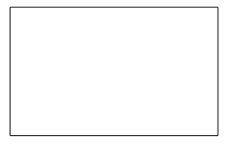
\includegraphics[width=0.3\textwidth]{fig-2-5.jpg}
	\caption{\label{fig:2-5}}
\end{figure}

黄金比很容易计算.
设正五边形的边长为$1$,对应的正五角星的边长为$x$,
那么黄金比就是$x$,满足
\[\frac{x}{1}=\frac{1}{x-1}\]
由此可得方程\[x^2-x-1=0\]
它的正解为
\[x=\frac{1+\sqrt{5}}{2}\approx 1.618.\]

线段$AC$的黄金分割可以很容易使用尺规作图得到(如图\ref{fig:2-6}所示).
作$AX$垂直于$AC$,使其长度为$AC$的一半.
以$X$为心、$XA$为半径作圆,交$XC$于$Y$.
再以$C$为心、以$CY$为半径作圆,交$AC$与$D'$.
那么点$D'$就是$AC$的黄金分割点.
这是因为,由勾股定理可知:
\[XC^2=AX^2+AC^2=AX^2+4AX^2=5AX^2.\]
因而
\[\frac{AC}{D'C}=\frac{2AX}{YC}=\frac{2AX}{XC-XY}=\frac{2AX}{\sqrt{5}AX-AX}
=\frac{2}{\sqrt{5}-1}=\frac{1+\sqrt{5}}{2}.\]
毕达哥拉斯学派很可能是知道黄金分割的这种几何结构的.

\begin{figure}[htbp]
	\centering
	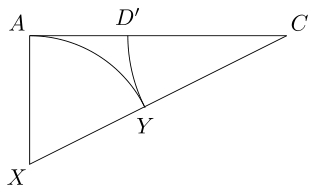
\includegraphics[width=0.3\textwidth]{fig-2-6.jpg}
	\caption{\label{fig:2-6}}
\end{figure}

请注意,上述构造方式也是一种构造正五边形的方式,
因为正五角星的角都是一种等腰三角形的顶角,
而这种等腰三角形的腰和底边之比正是黄金比.
所以,在毕达哥拉斯时代的希腊几何学家已经可以使用尺规作出正三角形、正方形、正五边形,
以及所有边数是上述正多边形边数二倍的正多边形.
后来,他们还发现了如何构造正15边形.由于$(2\times 3)-5=1$,
由此立即可得:
\[\frac{1}{15}=\frac{2\times3}{15}-\frac{5}{15}=\frac{2}{5}-\frac{1}{3}.\]
所以,要想将一个圆等分为15等份,只需要先作内接正五边形的两个连续的边从而获得圆周的2/5,
然后再作内接正三角形的一个边从而获得圆周的三分之一,二者相减即得圆周的1/15.

如果只考虑正多边形,这就是希腊几何学家所能作出的全部了.
直到两千年以后,高斯构造出了正十七边形,
这方面的工作才有了进一步的进展了.
同一时期,伽罗瓦及其他人在代数方程根式解方面的工作,
给出了尺规构造正多边形的充要条件.
但是如今我们仍然只知道六种可以通过尺规构造的基本正多边形,
它们的边数分别是3,4,5,17,257,65537!

\section{三等分角}

泰勒斯定理告诉我们如何将任意线段$AB$等分为$n$等份(如图\ref{fig:2-7}所示):
\begin{figure}[htbp]
	\centering
	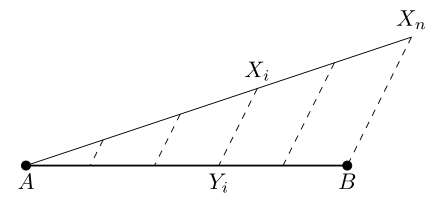
\includegraphics[width=0.4\textwidth]{fig-2-7.jpg}
	\caption{\label{fig:2-7}}
\end{figure}
\begin{itemize}
	\item 过点$A$作另一条直线;
	\item 在该直线上,从点$A$出发作$n$条等长的线段,记其分点分别为$X_1,\dots,X_n$;
	\item 连接$X_nB$;
	\item 过点$X_i$作$X_nB$的平行线;
	\item 记这些平行线与线段$AB$的交点依次为$Y_1,\dots,Y_{n-1}$,这就是$n$等分点.
\end{itemize}
所以接下来的一个很自然的问题就是:
\begin{framed}
	如何将任意一个角$n$等分?
\end{framed}
希腊几何学家当然会去尝试如何解决这个问题.
首先,将$\angle BAC$等分是很容易的(如图\ref{fig:2-8}所示):
\begin{figure}[htbp]
	\centering
	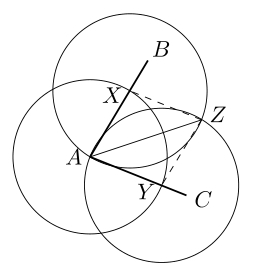
\includegraphics[width=0.25\textwidth]{fig-2-8.jpg}
	\caption{\label{fig:2-8}}
\end{figure}
\begin{itemize}
	\item 以$A$为心作圆,交$AB$于$X$,交$AC$于$Y$;
	\item 分别以$X$和$Y$为心、以$AX$和$AY$为半径作圆,交于$Z$;
	\item 由于$AXYZ$是菱形,所以对角线$AZ$平分$\angle BAC$.
\end{itemize}
所以下一步是如何将$\angle BAC$三等分:即所谓``三等分角问题''.
还是直到19世纪,才有人证明了这个问题在尺规作图下无解.

大约公元前420年,希庇亚斯提出了解决$n$等分角问题的如下方案(如图\ref{fig:2-9}所示):
\begin{figure}[htbp]
	\centering
	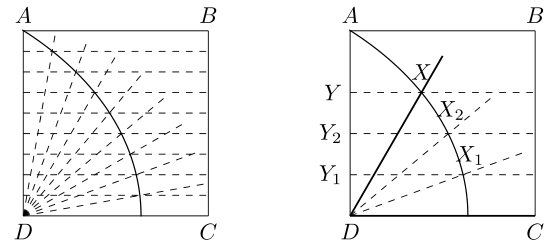
\includegraphics[width=0.5\textwidth]{fig-2-9.jpg}
	\caption{\label{fig:2-9}}
\end{figure}
\begin{itemize}
	\item 作正方形$ABCD$;
	\item 令边$DA$绕$D$匀角速度旋转至$DC$;
	\item 在等长的时间内,令边$AB$匀速下降至$DC$;
	\item 考虑两条运动线段的交点轨迹所成的曲线,这条曲线即希庇亚斯三分角线.
\end{itemize}
这条曲线的大部分都可以由此完美定义,
除了它的终点:
当两条动线段的运动结束时,其公共部分是线段$DC$本身!
但是这个对应于零度角的点与本问题无关.

显然,三分角线可以瞬间解决$n$等分$\angle XDC$的问题(如图\ref{fig:2-9}的右图所示,此时$n=3$).
\begin{itemize}
	\item 记$X$在$DA$上的投影为$Y$;
	\item 将线段$DY$等分为$n$份,设分点为$Y_i$;
	\item 过每个$Y_i$作$DC$的平行线,交三分角线于$X_i$;
	\item 那么,射线$DX_i$就将$\angle XDC$等分为$n$份.
\end{itemize}

但是,显然不可能通过尺规作图将三分角线的所有点都画出.
首先,存在无数多个点;
其次,并不是每个点都可以通过尺规构造:
例如,我们将在附录B的B.2节看到,20度角的对应点不能尺规作出.

希庇亚斯在公元前四世纪的这个构造,
似乎是已知最早的用于描述曲线(除了直线和圆之外)的数学语言.
而且还使用了一种动态方法进行描述.




\section{圆化方}

\begin{figure}[htbp]
	\centering
	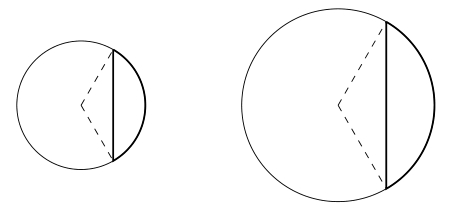
\includegraphics[width=0.5\textwidth]{fig-2-10.jpg}
	\caption{\label{fig:2-10}}
\end{figure}



\section{倍立方}

\section{不可公度量}

\section{穷竭法}

\section{关于空间的连续性}

\section{问题}

\section{练习}

\chapter{欧几里得的《原本》}

\section{卷一:直线}

\section{卷二:几何化的代数}

\section{卷三:圆}

\section{卷四:多边形}

\section{卷五:比例}

\section{卷六:相似性}

\section{卷七:算术中的除法}

\section{卷八:几何学的新进展}

\section{卷九:更多关于数的事情}

\section{卷十:不可公度量}

\section{卷十一:多面体几何}

\section{卷十二:穷竭法}

\section{卷十三:正多面体}

\chapter{几位希腊几何学大师}

\section{阿基米德关于圆的工作}

\section{阿基米德关于$\pi$的工作}

\section{阿基米德关于抛物线的工作}

\section{阿基米德关于螺旋线的工作}

\section{阿波罗尼乌斯关于圆锥曲线的工作}

\section{阿波罗尼乌斯关于共轭方向的工作}

\section{阿波罗尼乌斯关于切线的工作}

\section{阿波罗尼乌斯关于极点和极线的工作}

\section{阿波罗尼乌斯关于焦点的工作}

\section{海伦关于三角形的工作}

\section{梅涅劳斯关于三线共点的工作}

\section{托勒密关于三线共点的工作}

\section{帕普斯关于调和比的工作}

\section{问题}

\section{练习}

\chapter{后希腊时期的欧氏几何}

\section{对$\pi$的进一步探究}

\section{三角形的中位线}

\section{三角形的高}

\section{西瓦定理}

\section{三角形的三等分角线}

\section{再探圆锥曲线焦点}

\section{平面上的反演}

\section{多面体空间的反演}

\section{球极射影}

\section{烧掉直尺吧}

\section{问题}

\section{练习}

\chapter{射影几何}

\section{透视表示}

\section{射影几何vs欧氏几何}

\section{调和比}

\section{德萨格定理和帕普斯定理}

\section{公理化射影几何}

\section{德萨格平面和帕普斯平面}

\section{除环上的射影平面}

\section{希尔伯特定理}

\section{问题}

\section{练习}

\chapter{非欧几何}

\section{对欧几里得第五公设的探求}

\section{萨凯里四边形}

\section{三角形的内角}

\section{渐进平行线}

\section{三角形的面积}

\section{贝尔特拉米-克莱因圆盘和庞加莱圆盘}

\section{问题}

\section{练习}

\chapter{希尔伯特的公理化体系}

\section{关联公理}

\section{顺序公理}

\section{合同公理}

\section{连续公理}

\section{平行公理}

\section{问题}

\section{练习}


\bibliography{reference}

\appendix

\chapter{作图法}

\section{极小多项式}

\section{艾森斯坦因判别法}

\section{尺规作图}

\section{作图法与域论}

\chapter{古典问题}

\section{倍立方问题}

\section{三等分角问题}

\section{圆化方问题}

\chapter{正多边形}

\section{希腊几何学家们已经知道啥}

\section{问题代数化}

\section{费马数}

\section{同余基础}

\section{从伽罗瓦理论的视角来看}

\section{高斯-王策尔定理}

\end{document}
